% Part 2 chapter carrying "The Redshift-Dependent S8 Trend in the Context of IAM" (Mar 2026) in its order. Read in full 2026-10-02
% (323 lines, 50-line ledger). Numbers: docs/verification/scripts/verify_s8_trend.py. Check: docs/verification/observations/S8_TREND_CHECK.md.
% Naming rule: the compilation is cited by journal and arXiv number only.
\chapter{Growth across redshift: the $S_8$ trend}\label{ch:s8trend}

\section*{The place}
The cosmic horizon, where matter's records are written as it collapses into structure (Chapter~\ref{ch:surfaces}). The cost of writing weakens the
coupling felt by matter, $\mu<1$, and leaves light untouched, $\Sigma=1$. This chapter follows that weakening through the redshifts at which surveys
measure the clustering amplitude.

\section{The observation}
An analysis of redshift-space-distortion $f\sigma_8(z)$ measurements with $\Omega_m$ held to a Planck + BAO prior (\emph{MNRAS} 528, L20, 2024;
arXiv:\allowbreak{}2303.06928) finds that the inferred $S_8\equiv\sigma_8\sqrt{\Omega_m/0.3}$ rises with effective redshift: a $\sim3\sigma$ tension with the Planck
value of $0.832$~\cite{Planck2018VI} at lower redshifts becomes consistent within $1\sigma$ at high redshifts \observed. In $\Lambda$CDM, $S_8$ is one number at every redshift. The growth-index fit $f=\Omega_m(a)^\gamma$ to the same kind of data
gives $\gamma=0.633^{+0.025}_{-0.024}$ against $0.55$ in general relativity (Nguyen, Huterer and Wen 2023~\cite{Nguyen2023}).

\section{The coupling}
\begin{equation}\mu(a)=\frac{H^2(a)}{H^2(a)+\beta_mE(a)H_0^2},\qquad E(a)=e^{1-1/a},\qquad\beta_m=\Omega_m/2,\end{equation}
so $\mu(z{=}0)=0.864$, $\mu(0.5)=0.948$, $\mu(1)=0.982$, $\mu(2)=0.998$. The weakening is strongest today and gone by $z\approx2$: the shape of the
trend, with nothing adjusted.

\section{What a survey infers}

\begin{figure}[htbp]\centering
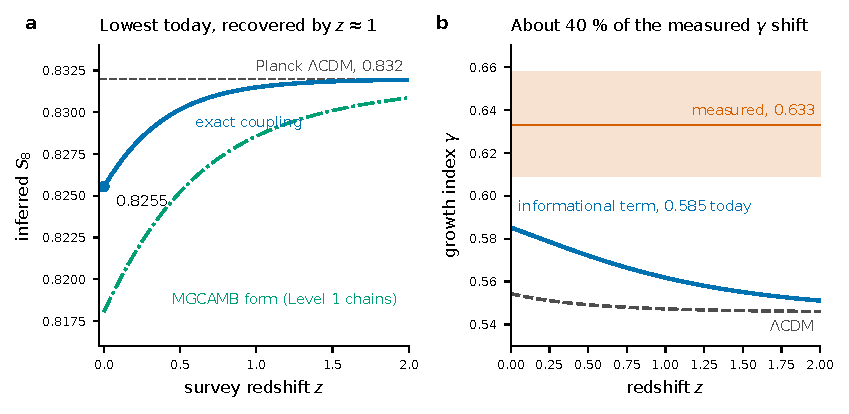
\includegraphics[width=\textwidth]{figures/part2/fig_s8_inferred.pdf}
\caption{(a) The $S_8$ a survey at redshift $z$ infers when it analyses with $\Lambda$CDM growth, $S_8^{\rm Planck}D_{\rm IAM}(z)/D_{\Lambda\rm CDM}(z)$, for the exact coupling (0.8255 today, a 0.78\,\% deficit) and for the MGCAMB form used in the Level~1 chains (1.68\,\% today); same early amplitude, Planck 2018 background. (b) The effective growth index $\gamma=\ln f/\ln\Omega_m(a)$: 0.585 today against 0.554 in $\Lambda$CDM \calc, and the measured $0.633^{+0.025}_{-0.024}$ (Nguyen, Huterer and Wen 2023, band) \observed.}\label{fig:s8_inferred}
\end{figure}
A survey measures the clustering amplitude at its redshift and, analysing with $\Lambda$CDM growth, reports $S_8$. The amplitude is the integrated
growth, not the instantaneous coupling: the inferred value is $S_8^{\rm Planck}\,D_{\rm IAM}(z)/D_{\Lambda\rm CDM}(z)$, from the linear growth equation
with the same early-time amplitude. ($S_8^{\rm Planck}\mu(z)$ treats a rate as an amount and overstates the effect about twentyfold.)
\begin{center}\small\begin{tabularx}{\linewidth}{>{\raggedright\arraybackslash}Xcccc}\toprule
$z$ & $\mu$ & inferred $S_8$ & deficit & $f_{\rm IAM}/f_{\Lambda\rm CDM}$\\\midrule
0 & 0.864 & 0.8255 & 0.78\,\% & 0.965\\ 0.25 & 0.914 & 0.8285 & 0.42\,\% & 0.980\\ 0.5 & 0.948 & 0.8302 & 0.22\,\% & 0.989\\
1.0 & 0.982 & 0.8315 & 0.06\,\% & 0.997\\ 2.0 & 0.998 & 0.8320 & 0.01\,\% & 1.000\\\bottomrule
\end{tabularx}\end{center}
The shape is the observed one: lowest today, recovering by $z\sim1$. The size is not. The predicted deficit today is $0.8\,\%$; the low-redshift weak-lensing surveys
sit $6$--$9\,\%$ below Planck~\cite{Asgari2021,DESY3}. The growth \emph{rate} is affected more than the amplitude: $f\sigma_8$ is $4.25\,\%$ low today \calc. The effective growth
index is $\gamma=0.585$ today ($0.572$ at $z=0.5$), against $0.554$ in $\Lambda$CDM and the measured $0.633$: about $40\,\%$ of the measured
departure.

\paragraph{The chain form.} The Level 1 chains used MGCAMB's form~\cite{Zhao2009MGCAMB,Wang2023MGCAMB} $\mu=1+\mu_0\Omega_{\rm DE}(a)/\Omega_{\rm DE,0}$, which equals the exact $\mu$
today but weakens growth more at $0.3<z<2$. The same integration with that form gives a $1.68\,\%$ amplitude deficit today, close to the chains'
$\sigma_8$ shift ($0.8143\to0.8015$, $1.6\,\%$, Planck alone) \calc. The exact form gives half of it.

\section{Light is unchanged}
With $\Sigma=1$ photons follow standard null geodesics, so BAO angles, the CMB acoustic scale and lensing geometry are those of $\Lambda$CDM. The
background is not modified: applying $\beta_m$ to the Friedmann equation gives $H_0\approx61.5$, excluded by every measurement, so the term acts on
matter perturbations only.

\section{Signatures}

\begin{figure}[htbp]\centering
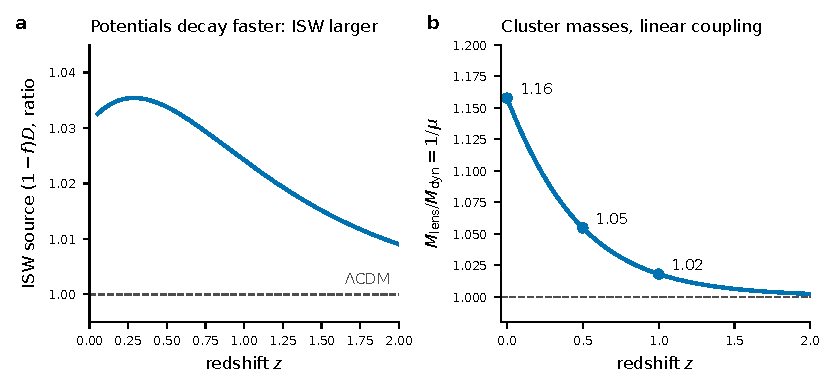
\includegraphics[width=\textwidth]{figures/part2/fig_growth_signatures.pdf}
\caption{(a) The ISW source $(1-f)D$ relative to $\Lambda$CDM with $\Sigma=1$: 3.4\,\% larger at $z\le0.5$. (b) $M_{\rm lens}/M_{\rm dyn}=1/\mu$ in the linear coupling: 1.16 today, 1.06 at $z=0.5$, 1.02 at $z=1$; whether the linear $\mu$ applies inside virialised clusters is open. Linear growth, same early amplitude. \prediction}\label{fig:growth_signatures}
\end{figure}
\begin{itemize}
\item \emph{Scale independence.} $\mu$ depends on $a$ only, so $P_{\rm IAM}(k)/P_{\Lambda\rm CDM}(k)$ is flat across survey scales; $f(R)$ growth is scale dependent~\cite{PogosianSilvestri2008}.
\item \emph{ISW.} With $\Sigma=1$ the lensing potential follows $\delta_m$, which grows more slowly, so the potentials decay faster: the ISW source
$(1-f)D/a$ is $3.4\,\%$ larger at $z\le0.5$, and the ISW--galaxy cross-correlation about $3\,\%$ larger. $f(R)$ predicts the opposite sign.
\item \emph{Cluster masses.} Lensing measures the mass; dynamics measures $\mu$ times it. In the linear coupling $M_{\rm lens}/M_{\rm dyn}=1/\mu$:
$1.16$ today, $1.06$ at $z=0.5$, $1.02$ at $z=1$. Whether the linear $\mu$ applies inside virialised clusters is open (Chapter~\ref{ch:threeway}) \openprob.
\item \emph{The $\mu$--$\Sigma$ plane.} $\mu_0=-0.136$, $\Sigma_0=0$. With conservative scale cuts Euclid is forecast to give $1+\mu_0$ to $23.3\,\%$ but $1+\Sigma_0$ to $2.6\,\%$~\cite{Albuquerque2025} \observed, so the
lensing half of the signature is the sharper test; a forecast for the full IAM $\mu(z)$ is open \openprob.
\end{itemize}

\section{Status}
Stands: the redshift shape of the weakening, the sector split, scale independence, the dated $\mu_0$. Calculated here \calc: the amplitude deficit the
informational term produces is $0.8\,\%$ today, about a tenth of the low-redshift deficit; the growth-rate deficit is $4.25\,\%$, and the growth index
moves $40\,\%$ of the way to the measured value. The $S_8$ trend is consistent in shape and smaller in size.
